\documentclass[12pt]{letter}
\usepackage[latin1]{inputenc}

\usepackage[left=1.00in, right=1.00in, top=1.00in, bottom=1.00in]{geometry}
\usepackage{amsmath}
\usepackage{amsfonts}
\usepackage{amssymb}
\usepackage[final]{pdfpages}
\address{Andrew Rosen  \\ Georgia State University \\  rosen@cs.gsu.edu} 
\signature{Andrew Rosen} 
\date{}
\begin{document} 
\begin{letter}{Department of Computer Science and Software Engineering \\University of Canterbury}
\opening{Dear Members of the Search Committee,} 
I am responding to your search for a lecturer position posted on your website.
I am currently a PhD candidate in the Department of Computer Science at Georgia State University, slated for graduation in May 2016.
I believe I can greatly contribute to your department's focus on computer science education and areas of research.

My research focuses on fault-tolerant systems, with an emphasis on P2P systems, distributed computing, and Big Data applications.
My research in distributed computing and networks will open up many avenues for collaboration with professors in your department who work in similar areas.
In addition, I have previously collaborated on Bioinformatics projects.



I am incredibly enthusiastic when it comes to teaching and have a strong teaching background.
I received the Outstanding Graduate Teaching award given by our Computer Science department in 2015.
I believe teaching both the practice of programming with an equal emphasis on the theoretical Computer Science and mathematical backgrounds of the subject give students the full understanding they need to succeed.




My research, my strong teaching record, and service background make me a strong candidate for the position.
I look forward to hearing from the search committee.


\closing{Thank you for your consideration,} 
%\cc{Cclist} 
%\ps{adding a postscript} 
%\encl{list of enclosed material} 
\end{letter} 
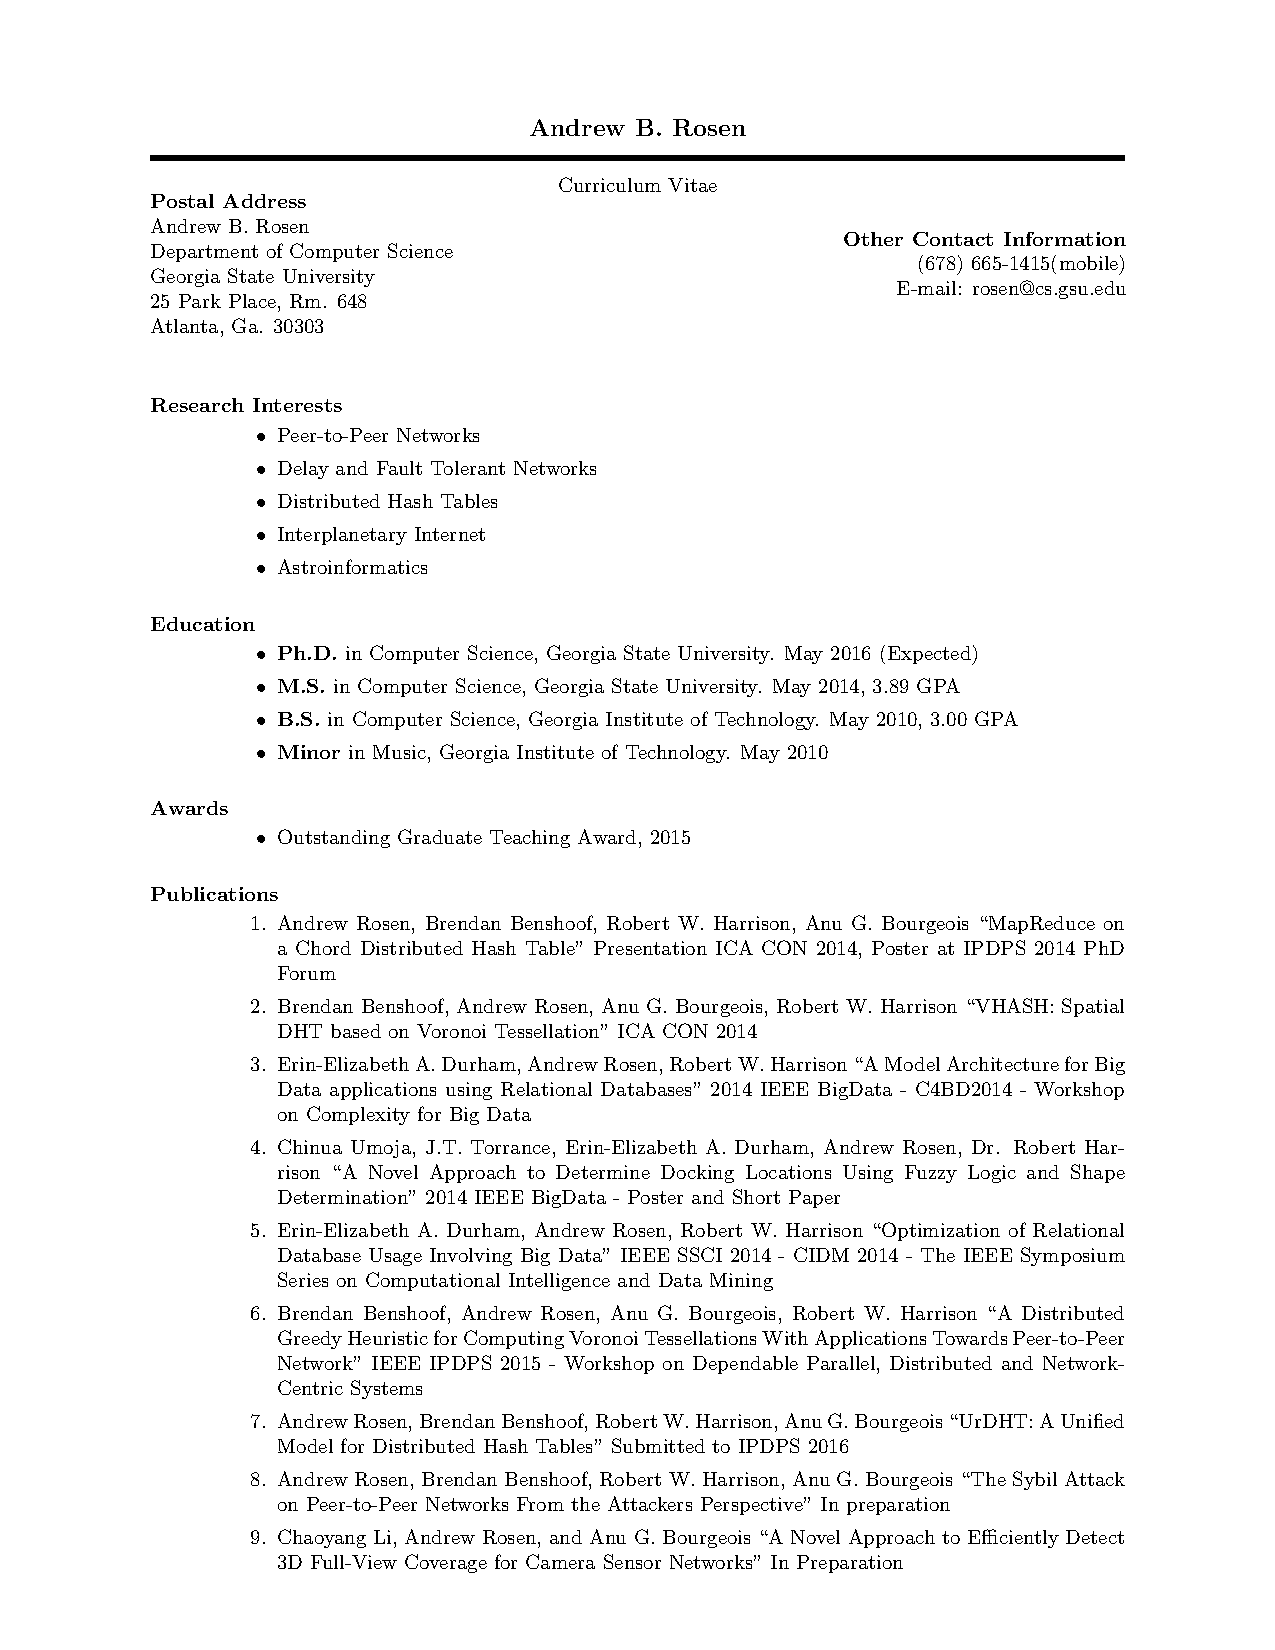
\includepdf[pages=-]{cv.pdf}
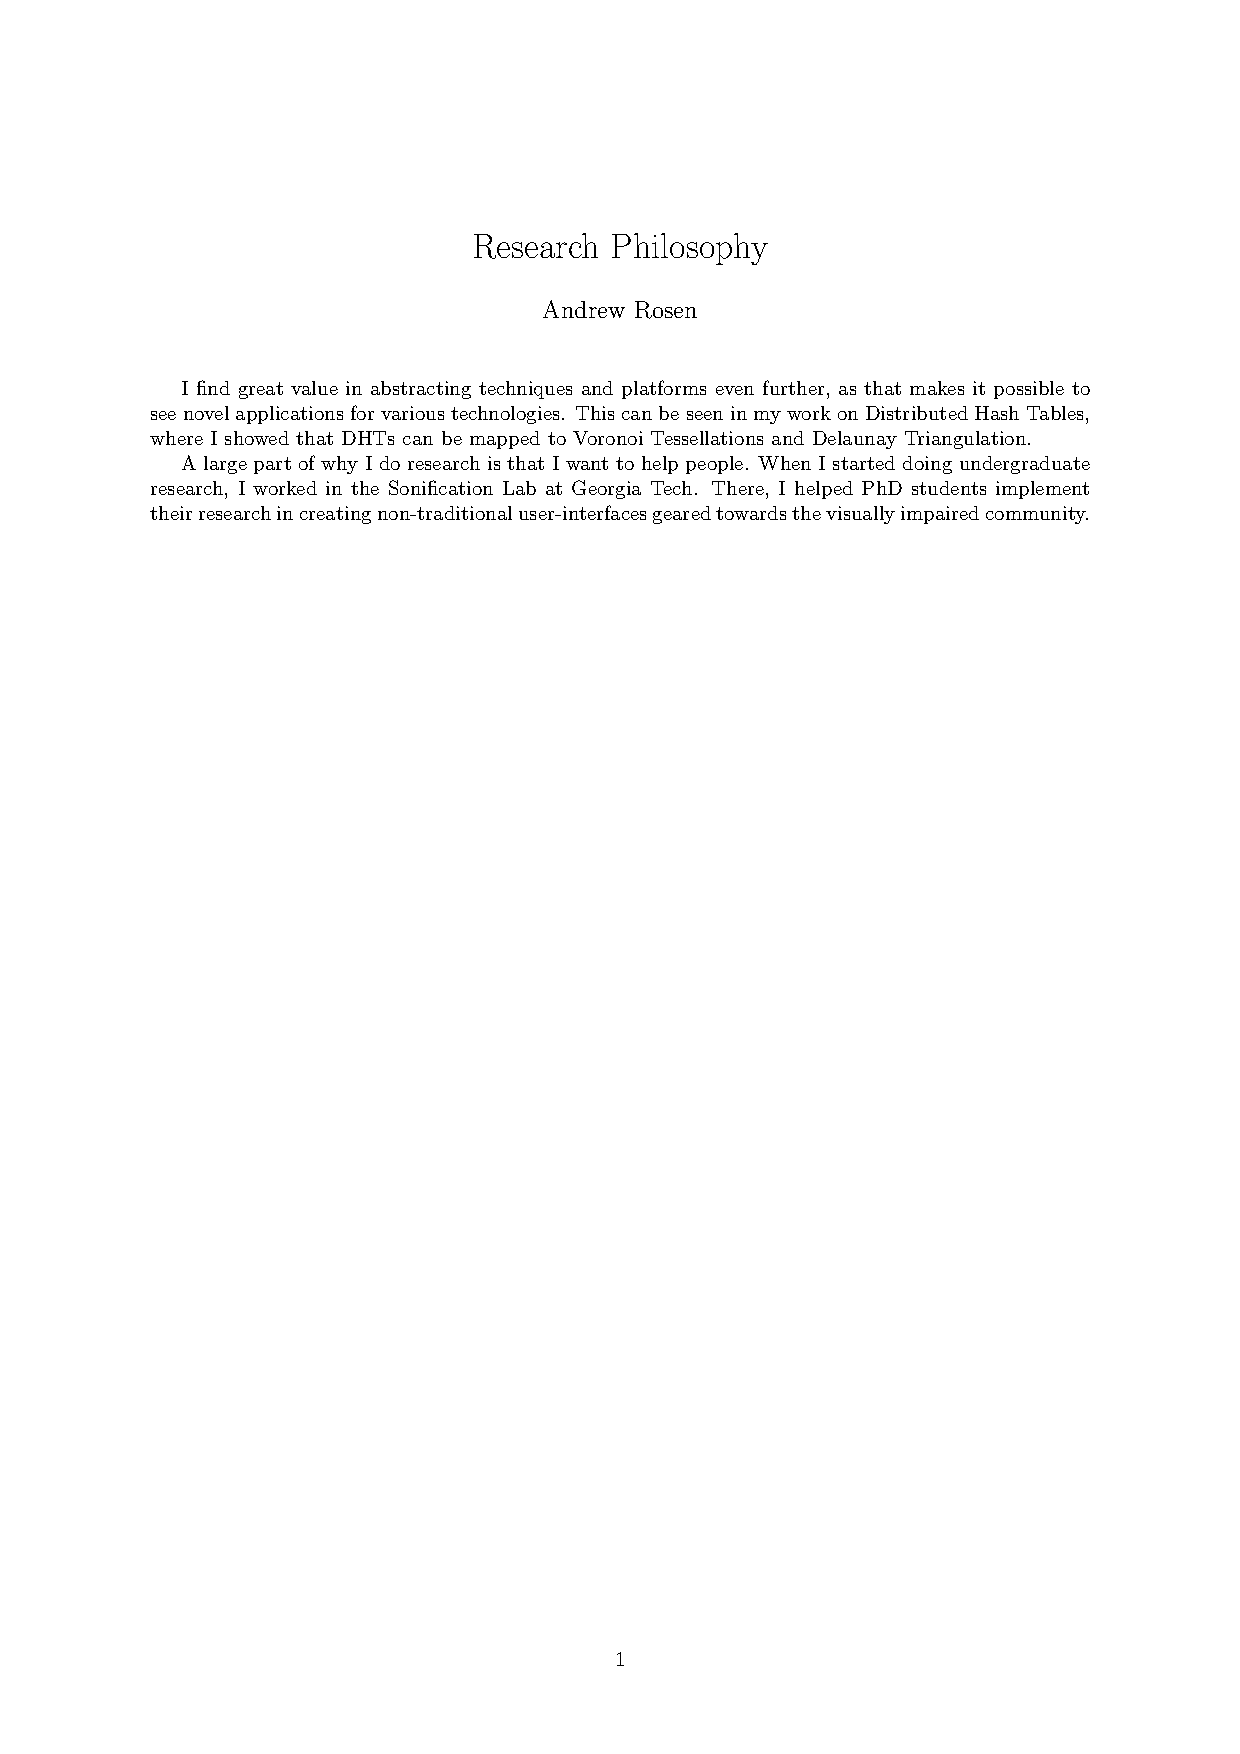
\includepdf[pages=-]{research.pdf}

\includepdf[pages=-]{teaching.pdf}

\end{document}
